\section{GPU-Accelerated Attribute Encoding/Decoding}\label{sec:gpu-raht}

In this section, we describe how we GPU-accelerate the encoding and decoding of Gaussian attributes, such as opacity, scale, rotation, and spherical harmonics.

\subsection{Background: RAHT}\label{sec:background-1}

Region-Adaptive Hierarchical Transform (RAHT) is an algorithm for encoding and decoding the attributes of sparse, spatially non-uniform data (such as point clouds~\cite{de2016compression} and \gs{} frames).
%
The algorithm is complex to explain in its entirety, so we use an example to explain the algorithm; details can be found in~\cite{de2016compression,raht}.
%% \ao{Include something like: interested readers can find a detailed description of RAHT in \cite{}. Eduardo: Is \cite{de2016compression} the most relevant reference here?}
%
To further simplify the description, we describe how it encodes a \textit{single attribute}, say opacity.

% \begin{figure}[t]
%   \centering
%     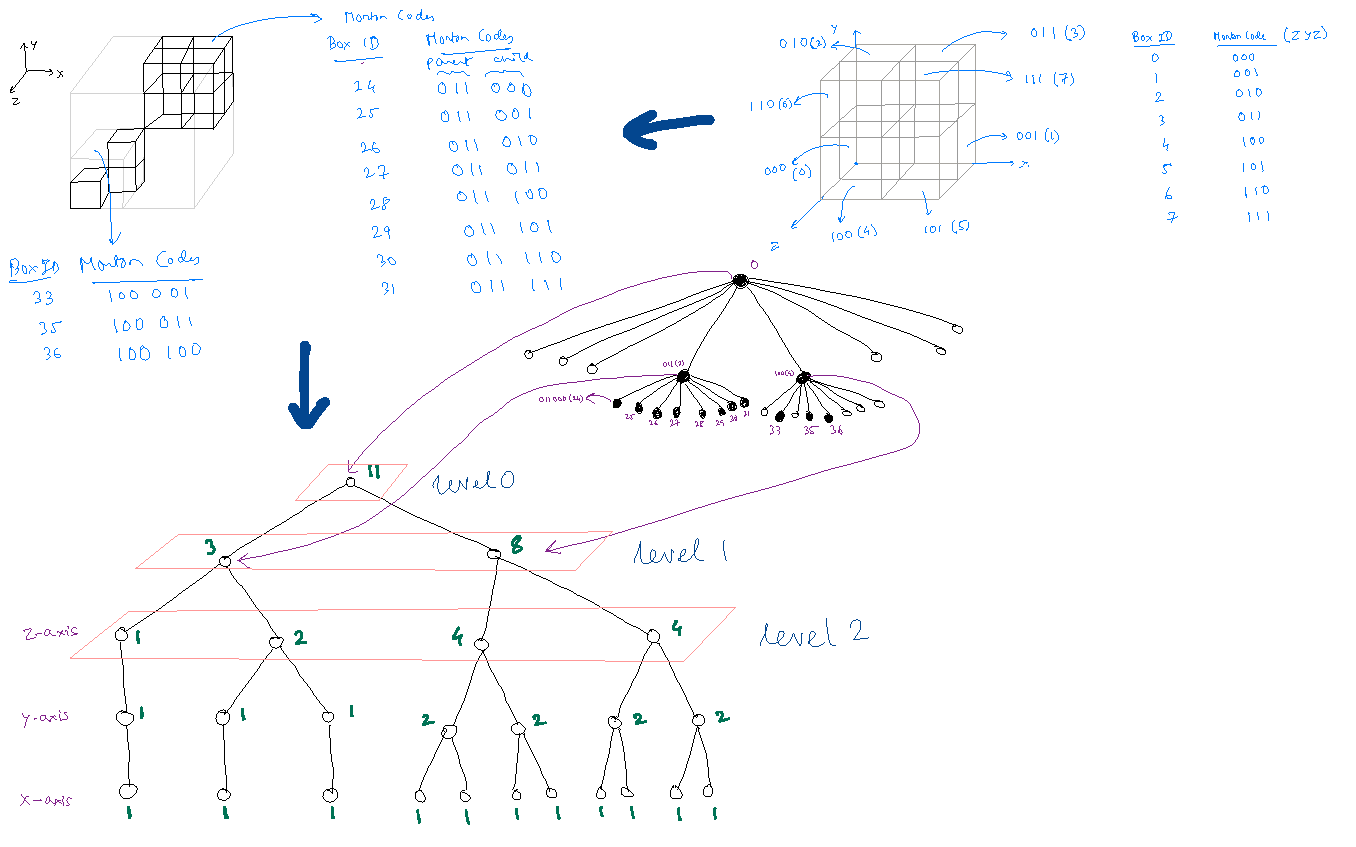
\includegraphics[width=\columnwidth]{figures/morton_code_octree_raht}
%     \caption{\label{fig:raht} Example to illustrate the RAHT algorithm.}
% \end{figure}
\begin{figure}[t]
  \centering
    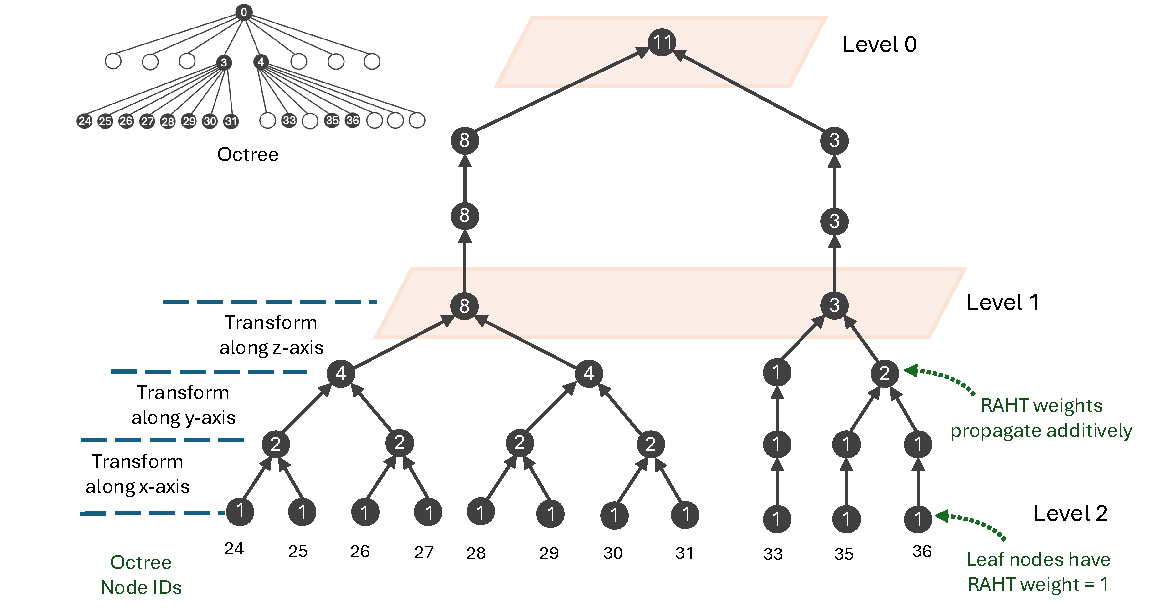
\includegraphics[width=\textwidth]{figures/raht_tree.pdf}
    \caption{Example to illustrate the RAHT algorithm.}
    \label{fig:raht} 
\end{figure}

RAHT exploits the octree structure derived from voxel positions (\cref{fig:raht}).
%
It operates on a binary tree derived from the octree; in this binary tree, each octree level is represented by 3 levels in the binary tree, each of which corresponds to one of the directional axes.
%
The leaves of the tree correspond to voxels, and in \cref{fig:raht} we only show branches in the binary tree leading to occupied voxels, for simplicity.

% \ramesh{Raj, please label tree nodes with box IDs as well, for ease of exposition.}

If a node has a sibling (\textit{e.g.}, nodes \textbf{35} and \textbf{36} in \cref{fig:raht}), RAHT decomposes the attribute into:
\begin{enumerate}
    \item \textbf{Low-frequency Coefficient:} A weighted average representing coarse signal information. 
    \item \textbf{High-frequency Coefficient:} A weighted difference representing the signal details.
\end{enumerate}
%
More precisely, if two siblings $l$ and $r$ have attribute values $a_l$ and $a_r$, then computing these coefficients requires a $2 \times 2$ matrix-vector multiplication:
%
\begin{equation}
  \begin{bmatrix}
  a^0\\
  a^1
  \end{bmatrix}
  =
  \frac{1}{\sqrt{w_l+w_r}}
  \begin{bmatrix}
  \sqrt{w_l} & \sqrt{w_r}\\
  -\sqrt{w_r} & \sqrt{w_l}
  \end{bmatrix}
  \begin{bmatrix}
  a_l\\
  a_r
  \end{bmatrix},
  \label{eq:raht-butterfly}
\end{equation}
%
In this equation, $a^0$ represents the low-frequency (coarse) coefficient, $a^1$ the high-frequency coefficient, and $w_l$ and $w_r$ represents \textit{weights} associated with $a_l$ and $a_r$ respectively.
%
The weight at any node is the number of occupied voxels in the octant below that node; attributes at leaf nodes have unit weights.
%
\cref{fig:raht} shows node weights next to the node.
%
RAHT propagates the low-frequency coefficient to the parent, while storing the high-frequency coefficients at the right sibling.
%
(If a node does not have a sibling such as node \textbf{33}, it passes its attribute value up to its parent).
%
RAHT then repeats this procedure level by level, bottom-up, on this tree.

At the end of this computation, the octree root stores the low-frequency component, and internal nodes and leaves store high-frequency coefficients.\footnote{This computation can be intuitively thought of as an extension of the Haar wavelet transform to a sparse 3D grid~\cite{de2016compression}.}
%
Smoothly varying spatial signals (\textit{e.g.}, point clouds can have smoothly varying color, just like images) have near-zero high-frequency coefficients, especially close to the leaves, which can be quantized and entropy-coded, resulting in significant compression.
%
In \gsnfs{}, we use RAHT to encode all \gs{} attributes (\cref{sec:3d-gauss-splatt}) other than positions.
%
RAHT decoding inverts this operation; for brevity, we discuss only the RAHT encoder and leave the decoder (inverse-RAHT) to~\cref{app:sysn-raht-encod}.

\subsection{Background: A Re-formulated RAHT Algorithm}\label{sec:backgr-fast-raht}

%% \ao{Can we come up with an acronym for "Pavez et al's reformulation of the original RAHT algorithm"? It could be P-RAHT, P for prelude, and for Pavez :), and it would be easier to use later in the text, instead of "Pavez et al's reformulation of RAHT" which is used multiple times below.}

Pavez \textit{et al.}~\cite{raht} describe a re-formulation (henceforth P-RAHT) of the original RAHT algorithm~\cite{de2016compression} that exploits properties of the Morton code.
%
P-RAHT takes as input occupied voxels and their associated Morton codes.
%
It pre-computes, in a step called the \textit{RAHT} prelude, the constructs needed for the hierarchical RAHT computation, the sibling relationships and the node weights, since these are a function of voxel occupancy alone, not of the attribute.
%
Then, it re-uses these when encoding each attribute.

%% \begin{figure}[t]
%%   \centering
%%     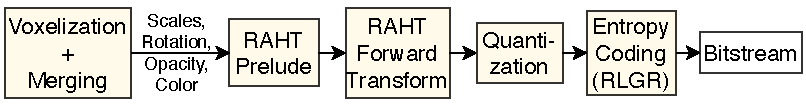
\includegraphics[width=\columnwidth]{figures/raht_pipeline.pdf}
%%     \caption{RAHT coding pipeline.\eduardo{This figure should have the KLT.}}
%%   \label{fig:raht-pipeline}
%% \end{figure}

\parab{The RAHT prelude.}
%
This step computes three lists at every level $\ell \in \{1,\dots,3J\}$:
%
(i) an index list $I_\ell$ indicating those nodes in the binary tree at level $\ell$ that are either left siblings, or singletons (those with no occupied siblings); (the binary tree in \cref{fig:raht} shows only the nodes in these lists)
%
(ii) a weight list $W_\ell$ for those nodes (indicated by numbers inside nodes in \cref{fig:raht}, and
%
(iii) a flag list $F_\ell$ indicating which nodes are left siblings (not shown in the figure for brevity).

P-RAHT computes these lists bottom-up.
%
Consider a node $n$ at level $\ell$.
%
Its weight is the sum of the weights of its children at level $\ell+1$.
%
If either of its children is in $I_{\ell+1}$, node $n$ must be in $I_{\ell}$.
%
Finally, if $n$'s sibling at level $\ell$ is also in $I_{\ell}$, it is the left sibling if it has a lower Morton code.
%
For example, the rightmost node at the second level from the bottom has a weight of 2, because its children are both occupied.
%
For that reason as well, it belongs in the $I_\ell$ list for that level.
%
But, it does not belong in the corresponding $F_\ell$ list, since it is \textit{not} the left sibling at that level.
%\eduardo{missing sub indicies $\ell$ in F and I above?}

\parab{Computing RAHT Coefficients.}
%
Using these lists, P-RAHT computes the RAHT coefficients using another bottom-up pass for each attribute.
%
If a node $n$ at level $\ell$ is a left sibling (\textit{i.e.}, its flag is set in $F_\ell$), then it computes the low-frequency and high-frequency coefficients using~\cref{eq:raht-butterfly}.
%
Nodes \textbf{24} and \textbf{35} in \cref{fig:raht} are examples of left siblings.
%
It then passes the low-frequency coefficient to its parent and stores the high-frequency attribute in its right sibling.
%
For this, it uses the pre-computed weights in $W_\ell$.
%
If $n$ is a singleton, such as node \textbf{33} in \cref{fig:raht}, it simply passes its attribute to its parent.

\subsection{GPU-Accelerated RAHT}\label{sec:gpu-accelerated-raht}

%% \begin{outline}
  
%%   \begin{itemize}
%%   \item inputs and outputs
%%   \item key idea: an alternative RAHT algorithm and the template established for octree, as well as vectorized attributes.
%%   \end{itemize}

%%   Template
%%   \begin{itemize}
%%   \item Use morton codes to avoid pointer chasing
%%   \item Bottom up or top-down computations level by level
%%   \item At each level, create as many GPU threads as needed, one for each node involved in the computation
%%   \item To find these nodes, use a pre-computation pass (draw examples from octree)
%%   \end{itemize}

%%   High-level: Pavez et al.'s reformulation has exactly the properties we need to parallelize RAHT.

%%   Describe how we compute the prelude: what GPU operations we use etc.
%%   RAHT itself is straightforward, show how we use the lists.
  
%% \end{outline}

\parab{Inputs and Outputs.}
%
\gsnfs{}'s GPU-accelerated RAHT takes as input occupied voxels, their Morton codes, and the attributes of the merged Gaussian in the voxel.
%
It outputs RAHT coefficients for all attributes.

\parab{Key Ideas.}
%
Our GPU-accelerated RAHT relies on three observations.
%
First, we observe that the basic RAHT algorithm is similar to the octree construction, encoding and decoding algorithms (\cref{sec:gpu-octree}).
%
RAHT proceeds bottom-up on a tree, performing one or more computations at some but not all nodes (\textit{e.g.}, only siblings), at each level in the tree.
%
The same is true for octree construction (\cref{sec:octree-encode-gpu}), for example, which performs computations only occupied nodes at each level.

This suggests that we can compute RAHT coefficients using the following design elements from those algorithms.
%
(a) Those algorithms use properties of Morton codes to mitigate compute stalls due to pointer chasing.
%
(b) They proceed sequentially level-by-level bottom-up or top-down, but within a level, they launch one GPU thread for every node in the tree involved in the computation.
%
(c) The set of nodes at a level involved in the computation is of variable length, so these algorithms employ PyTorch~\cite{pytorch} operations to convert fixed length vectors to variable length ones.
%
For example, the octree construction algorithm first creates a list of all occupied parents, then uses the \texttt{unique} operation to identify exactly the set of nodes at the next higher level involved in determining occupied nodes.

Our second observation is that P-RAHT is an ideal starting point for parallelization.
%
In particular, the pre-computed lists from the RAHT prelude greatly simplify applying the design elements described above.

Our third observation is that GPUs allow us to trivially \textit{parallelize RAHT coefficient computation across attributes}.
%
We can simply vectorize the attributes, and compute the coefficients in one bottom-up pass.

\parab{Computing RAHT coefficients on the GPU.}
%
\gsnfs{} computes RAHT coefficients bottom-up, exactly like P-RAHT.
%
Unlike P-RAHT, at each level, it launches multiple GPU threads.
%
Specifically, at level $\ell$, it launches a GPU kernel with one thread per entry in the list $I_\ell$.
%
For example, at the lowest level in \cref{fig:raht}, \gsnfs{} will launch \textbf{11} threads, and at the next level up, \textbf{7}.
%
Only threads whose flag $F_\ell$ is valid execute the $2\times2$ transform; each such thread reads indices of a sibling pair (current and next element in $I_\ell$), looks up their weights in $W_\ell$, and then applies Eq.~\ref{eq:raht-butterfly} to the attributes.

\parab{Parallelizing the RAHT Prelude.}
%
At each step $\ell$, \gsnfs maintains the current active list $I_\ell$ as a flat GPU tensor of indices.
%
We launch one GPU thread per element of $I_\ell$ to compute $W_\ell$ and $F_\ell$.
%
Each thread compares the Morton code of its current element with the next element (adjacent in Morton order) to decide whether they form a sibling pair.

After $F_\ell$ is computed, \gsnfs{} obtains the next active list $I_{\ell+1}$  by removing right siblings.
%
It implements this efficiently using boolean shift and masked select of tensors which are available in PyTorch (Alg.~\ref{algo:raht-prelude-gpu}).
%
The output of this is a compacted list containing exactly the set of nodes at $\ell+1$ that should run the RAHT coefficient computation at that level.

Especially for accelerating RAHT on a mobile GPU, we have found it essential to implement some of these steps using CUDA (\cref{sec:evaluation}).

\parab{Detailed Algorithm.}
%
We implement RAHT as a two-stage GPU pipeline: a \emph{prelude} that builds the merge schedule from Morton-sorted occupied voxels, and a \emph{transform} stage that applies the weighted orthonormal rotations using that schedule. This separation isolates the octree-dependent control flow from the per-attribute transform, allowing the latter to be executed with simple parallel kernels.

\begin{algorithm}[t!]
  \caption{RAHT prelude (non-parallel)}
  \label{algo:raht-prelude}
\SetAlgoLined
\DontPrintSemicolon
\SetKwInOut{Input}{Input}
\SetKwInOut{Output}{Output}

\Input{Morton codes $M[0{:}N_v{-}1]$, Num voxels $N_v$, octree depth $J$}
\Output{$[(I_\ell, W_\ell, F_\ell)]_{\ell=1}^{3J}$}

\For{$\ell \gets 1$ \KwTo $3J$}{
  \uIf{$\ell = 1$}{
    $I_1 \gets (0{:}N_v{-}1)^{T}$ \tcp*{active indices at level 1}
  }\Else{
    $I_\ell \gets I_{\ell-1}\big(\neg [0; F_{\ell-1}]\big)$ \tcp*{keep left siblings + singletons}
  }
  $M_\ell \gets M[I_\ell]$ \tcp*{Morton codes at level $\ell$}
  $W_\ell \gets [I_\ell(2{:}\mathrm{end});\, N_v] - I_\ell$ \tcp*{run-length weights (sentinel $N_v$)}
  $D \gets M_\ell(1{:}\mathrm{end}{-}1)\ \oplus\ M_\ell(2{:}\mathrm{end})$ \tcp*{path diffs}
  $F_\ell \gets \big(D\ \wedge\ (2^{3J} - 2^{\ell})\big) = 0$ \tcp*{left-sibling flags}
}
\Return $[(I_\ell, W_\ell, F_\ell)]_{\ell=1}^{3J}$\;
\end{algorithm}

Algorithm~\ref{algo:raht-prelude} gives the reference non-parallel prelude. For each of the $3J$ binary merge steps induced by a depth-$J$ octree, it constructs the active index list $I_\ell$, the corresponding run-length weights $W_\ell$, and the sibling flags $F_\ell$. Here, $W_\ell$ records the number of original voxels represented by each active entry, and $F_\ell$ marks whether an entry is the left element of a valid sibling pair. The sibling relation is tested directly from Morton codes using XOR and a level-dependent mask, without explicitly materializing the octree.

\begin{algorithm}[t!]
  \caption{RAHT Prelude on GPU}
  \label{algo:raht-prelude-gpu}
\SetAlgoLined
\DontPrintSemicolon
\SetKwInOut{Input}{Input}
\SetKwInOut{Output}{Output}
\SetKwFunction{Shift}{torch.shift}
\SetKwFunction{MaskedSelect}{torch.masked\_select}
\SetKwFunction{FWKernel}{FWKernel}

\Input{Morton codes $M[0{:}N_v{-}1]$, Num voxels $N_v$, octree depth $J$}
\Output{$[(I_\ell, W_\ell, F_\ell)]_{\ell=1}^{3J}$}

$I_1 \gets (0{:}N_v{-}1)^{T}$\;
\For{$\ell \gets 1$ \KwTo $3J$}{
  $\mu_\ell \gets (2^{3J} - 2^{\ell})$ \tcp*{mask for sibling test}
  % $end \gets N_v$ \tcp*{sentinel for run-length weights}
  \ForPar(\tcp*[f]{1 GPU thread per $k$}){$k \gets 1$ \KwTo $M_\ell$}{
    $curr \gets I_\ell(k)$\;
    $next \gets \begin{cases}
      end & \text{if } k = M_\ell\\
      I_\ell(k{+}1) & \text{otherwise}
    \end{cases}$\;

    $W_\ell(k) \gets next - curr$\;

    \uIf{$k = M_\ell$}{
      $F_\ell(k) \gets 0$\;
    }\Else{
      $F_\ell(k) \gets ((M(curr) \oplus M(next)) \wedge \mu_\ell ) = 0$\;
    }
  }

  $P_\ell \gets \Shift(F_\ell)$ \tcp*{$[0; F_\ell(0{:}\mathrm{end}{-}1)]$ marks right siblings}
  $I_{\ell+1} \gets \MaskedSelect(I_\ell, \neg P_\ell)$

  \If{$|I_{\ell+1}| = 1$}{
    % $L \gets \ell$\;
    \textbf{break}\;
  }
}
\Return $[(I_\ell, W_\ell, F_\ell)]_{\ell=1}^{3J}$\;
\end{algorithm}

Algorithm~\ref{algo:raht-prelude-gpu} shows the GPU version of this schedule construction. At each level, one thread computes the weight and sibling flag for one active entry. The next active list is then obtained by removing right siblings while keeping left siblings and singletons. This produces the schedule $[(I_\ell, W_\ell, F_\ell)]_{\ell=1}^{3J}$ used by the transform.

Algorithm~\ref{algo:raht-forward} applies the forward or inverse RAHT on the GPU. In the forward pass, levels are processed bottom-up; in the inverse pass, they are processed in reverse order. For each sibling pair, the transform uses the standard RAHT weights
$$
a=\sqrt{\frac{w_0}{w_0+w_1}}, \qquad
b=\sqrt{\frac{w_1}{w_0+w_1}},
$$
to perform the corresponding orthonormal rotation independently for each attribute channel. Since pairs within a level are disjoint, the computation can be parallelized across active entries.

\clearpage
\begin{algorithm}[p]
  \caption{RAHT Transform (Forward / Inverse) on GPU}
  \label{algo:raht-forward}
  \SetAlgoLined
  \DontPrintSemicolon
  \SetKwInOut{Input}{Input}
  \SetKwInOut{Output}{Output}
  
  \Input{Attributes $A\in\mathbb{R}^{N_v\times C}$ (GPU), prelude schedule $[(I_\ell,W_\ell,F_\ell)]_{\ell=1}^{3J}$, \texttt{inverse} flag}
  \Output{Coefficients $Y\in\mathbb{R}^{N_v\times C}$ (GPU)}
  
  $Y \gets A$ \tcp*{clone for in-place updates}
  \If{\texttt{inverse} = 0}{
    \For(\tcp*[f]{bottom-up}){$\ell \gets 1$ \KwTo $3J-1$}{
      $M_\ell \gets |I_\ell|$\;
      Launch \texttt{raht\_forward\_level\_kernel} with $M_\ell$ threads\;
      \Indp
      \ForPar{$k \gets 0$ \KwTo $M_\ell-2$}{
        \If{$F_\ell[k]$}{
          $i_0 \gets I_\ell[k]$;\;
          $i_1 \gets I_\ell[k+1]$;\;
          $w_0 \gets W_\ell[k]$;\;
          $w_1 \gets W_\ell[k+1]$;\;
          $a \gets \sqrt{w_0/(w_0+w_1)}$;\;
          $b \gets \sqrt{w_1/(w_0+w_1)}$;\;
          \For{$c \gets 0$ \KwTo $C-1$}{
            $y_0 \gets Y[i_0,c]$;\;
            $y_1 \gets Y[i_1,c]$;\;
            $Y[i_0,c] \gets a\cdot y_0 + b\cdot y_1$\;
            $Y[i_1,c] \gets -b\cdot y_0 + a\cdot y_1$\;
          }
        }
      }
      \Indm
    }
  }{
    \For(\tcp*[f]{top-down}){$\ell \gets 3J-1$ \KwTo $1$}{
      $M_\ell \gets |I_\ell|$\;
      Launch \texttt{raht\_inverse\_level\_kernel} with $M_\ell$ threads\;
      \Indp
      \ForPar{$k \gets 0$ \KwTo $M_\ell-2$}{
        \If{$F_\ell[k]$}{
          $i_0 \gets I_\ell[k]$;\;
          $i_1 \gets I_\ell[k+1]$;\;
          $w_0 \gets W_\ell[k]$;\;
          $w_1 \gets W_\ell[k+1]$;\;
          $a \gets \sqrt{w_0/(w_0+w_1)}$;\;
          $b \gets \sqrt{w_1/(w_0+w_1)}$;\;
          \For{$c \gets 0$ \KwTo $C-1$}{
            $y_0 \gets Y[i_0,c]$;\;
            $y_1 \gets Y[i_1,c]$;\;
            $Y[i_0,c] \gets a\cdot y_0 - b\cdot y_1$\;
            $Y[i_1,c] \gets b\cdot y_0 + a\cdot y_1$\;
          }
        }
      }
      \Indm
    }
  }
  \Return $Y$\;
\end{algorithm}
\clearpage

% \begin{algorithm}[t]
%   \caption{\textsc{FWKernel}: Compute $(W_\ell,F_\ell)$ on GPU}
%   \label{algo:raht-fwkernel}
% \SetAlgoLined
% \DontPrintSemicolon
% \SetKwInOut{Input}{Input}
% \SetKwInOut{Output}{Output}

% \Input{Index list $I_\ell$ (len $M_\ell$), Morton codes $M$, mask $\mu_\ell$, end sentinel $end$}
% \Output{Weights $W_\ell$ (len $M_\ell$), Flags $F_\ell$ (len $M_\ell$)}

% \ForPar(\tcp*[f]{1 GPU thread per $k$}){$k \gets 1$ \KwTo $M_\ell$}{
%   $curr \gets I_\ell(k)$\;
%   $next \gets \begin{cases}
%     end & \text{if } k = M_\ell\\
%     I_\ell(k{+}1) & \text{otherwise}
%   \end{cases}$\;

%   $W_\ell(k) \gets next - curr$\;

%   \uIf{$k = M_\ell$}{
%     $F_\ell(k) \gets 0$\;
%   }\Else{
%     $F_\ell(k) \gets ((M(curr) \oplus M(next)) \wedge \mu_\ell ) = 0$\;
%   }
% }
% \Return $(W_\ell,F_\ell)$\;
% \end{algorithm}



\subsection{Quantization and Entropy Coding}\label{sec:quant-entr-coding}

After obtaining the RAHT coefficients for each attribute, \gsnfs{} \textit{quantizes} these coefficients.
%
Quantization trades off visual quality by reducing the number of bits required to represent a coefficient.
%
We quantize coefficients of different \gs{} attributes to different levels, similar to~\cite{mesongs,gpcc-adaptive}.
%
\gsnfs{} uses dead-zone quantization~\cite{deadzone}, which is simple to implement on a GPU, using one thread per coefficient, and vectorizing the attributes.

\gsnfs{} uses an entropy coder to efficiently serialize quantized coefficients into a bitstream.
%
We use the Run-Length Golomb-Rice (RLGR)~\cite{rlgr} entropy coder, which uses run-length coding for consecutive zeros, and Golomb-Rice coding for non-zero magnitudes using an adaptive parameter.
%
%% \ao{It's unclear to me how the blocks are created. I assume the RAHT coefficients for an attribute are generated as a vector, and then this vector is divided into blocks?}
RLGR is inherently sequential, but \gsnfs{} parallelizes this by dividing the vector of coefficients, and entropy coding \textit{blocks} (\textit{e.g.}, 2K or 4K successive coefficients) using one GPU thread per block.
%
This ensures fast entropy coding at the expense of a slight loss in compression efficiency.

We have omitted a discussion of de-quantization and entropy decoding for brevity; \gsnfs{} also parallelizes this.
%
Thus, in \gsnfs{}, \textit{all steps} in octree and attribute encoding are GPU-accelerated.
%
%This is essential for avoiding CPU-GPU memory transfer overheads.

%% \parab{GPU-parallel RLGR: block-based parallelism.}
%% Since all previous stages of \gsnfs runs on GPU, it is critical to implement RLGR encoding and decoding on GPU as well to avoid costly CPU-GPU data transfers.
%% %
%% But, RLGR is inherently sequential \emph{within a stream} due to its adaptive state.
%% %
%% \gsnfs addresses this by encoding in blocks and running independent RLGR for each block in parallel.
%% %
%% We treat the coefficient matrix as $D$ independent channels, each of length $N_v$ symbols, and partition each channel into fixed-size blocks of $B$ (block size) symbols.
%% %
%% Each (channel, block) pair is encoded in parallel.
%% %
%% Such block-based parallelism achieve lower compression gain than encoding the entire channel, but we found this overhead to be small enough to tradeoff for improved runtime.


%% \begin{comment}


%% %% RAHT can be applied to any attributes of a point cloud, typically it is applied to color. 
%% %% %
%% %% We show that RAHT can also be effective for compressing \gs attributes including opacity, scale, rotation, and color (represented as spherical harmonics).

%% %% It can be intuitively understood as an extension of the  Haar wavelet transform to a sparse 3D grid.

%% %
%% % RAHT is even more effective for \gs since it allows high compressibility for all these attributes using entropy coding.

%% \parab{RAHT prelude.}
%% \eduardo{I would move this to the other section. The prelude was not in the original RAHT paper from  (de Queiroz and chou), that I added earlier.  When you introduce the parallel RAHT, you can mention the prelude and say that we need this new approach to effectively parallelize RAHT.}
%% %
%% In the original RAHT formulation, the transform is strictly dependent on the siblings of each node in the octree.
%% %
%% A parent node in the octree might have anywhere from one to eight occupied children.
%% %
%% The prelude step must scan the grid and identify which nodes are siblings.
%% %
%% If a node is the only child, it has no sibling, and its value is promoted without transformation.
%% %
%% If multiple siblings exist, they must be paired.
%% %
%% The RAHT prelude is pre-processing step that helps finding sibling pairs with corresponding weights for the RAHT transform.

%% \subsection{Parallelized RAHT}\label{sec:raht-encode-gpu}
%% \begin{figure}[t]
%%   \centering
%%     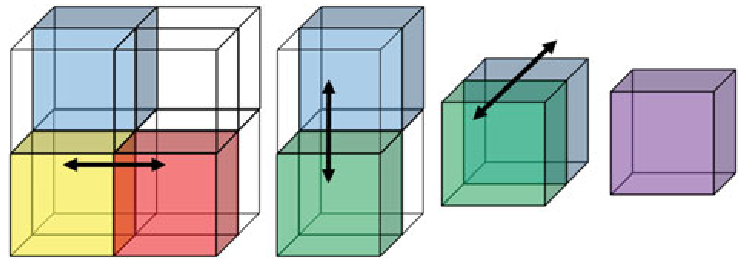
\includegraphics[width=\columnwidth]{figures/raht.png}
%%     \caption{One level of RAHT applied to eight adjacent voxels (colored are occupied). \raj{Replace it with binary tree figure}}
%%   \label{fig:raht}
%% \end{figure}
%% %
%% A \gs frame contains a set of Gaussians (one per occupied voxel), each having attributes such as scale, rotation, opacity, and color.
%% %
%% For degree 3 SH, there will be $3 + 4 + 1 + 48 = 56$ attributes that.
%% %
%% These attributes are spatially correlated: neighboring voxels often have similar opacity and geometry attributes, and smooth surfaces induce slowly varying SH coefficients.
%% %
%% Naively entropy coding the raw attributes waste bits because it ignores this correlation, leading to poor compression efficiency.
%% %
%% To exploit spatial correlation, \gsnfs applies a transform coder---analogous to DCT/wavelets in 2D video---that concentrates most attribute energy into a small number of low-frequency coefficients and produces many near-zero high-frequency residuals that are highly compressible.
%% %
%% G-PCC applies uses  RAHT-based transform coding for voxelized point attributes such as color. 
%% %
%% Similarly, for each 3DGS we build the RAHT on top of the voxelized geometry and apply it to the remaining \gs attributes. 
%% %
%% RAHT applies a sequence of orthonormal $2\times 2$ transforms to attributes living on the \emph{occupied} leaf voxels, proceeding bottom-up from leaves to the root; the inverse transform runs in the reverse order.\eduardo{this paragraph above describing 2x2 transforms can be moved to the how raht works subsection below.}

%% \parab{How RAHT works.}
%% We illustrate the forward RAHT using the canonical example in Fig.~\ref{fig:raht}. 
%% %
%% Consider a $2 \times 2 \times2$ cube where only three of the eight voxels are occupied (colored voxels in the figure). 
%% %
%% The attribute (say opacity) in three colored voxels has values $a_r,a_y,a_b$ (red, yellow, and blue, respectively) and an initial unit weight of $w_r,w_y,w_b$.
%% %
%% At a certain level in the octree, RAHT processes sibling voxel pairs axis-by-axis ($x$, then $y$, then $z$). If a voxel has no neighbor along the current axis, its coefficient is copied forward unchanged \eg the blue voxel in the $x$-axis.
%% %
%% Note that attribute values are only located at leaf, so RAHT applies the transform bottom-up from leaf level to root.
%% %
%% \raj{Mark the 3D axes in the figure and show the axis-by-axis processing.}
%% %
%% If two neighbors exist \eg red and yellow, RAHT applies the orthonormal transform, given by the equation:
%% \begin{equation}
%%   \begin{bmatrix}
%%   a_g^0\\
%%   a_g^1
%%   \end{bmatrix}
%%   =
%%   \frac{1}{\sqrt{w_y+w_r}}
%%   \begin{bmatrix}
%%   \sqrt{w_y} & \sqrt{w_r}\\
%%   -\sqrt{w_r} & \sqrt{w_y}
%%   \end{bmatrix}
%%   \begin{bmatrix}
%%   a_y\\
%%   a_r
%%   \end{bmatrix},
%%   \label{eq:raht-butterfly}
%% \end{equation}
%% where $a_g^0$ is the low-frequency (coarse) coefficient and $a_g^1$ is the high-frequency (detail) coefficient.
%% %
%% After the transform, both coefficients will have updated weights $w_g = w_y + w_r$ (green cube). 
%% %
%% The coefficient $a_g^1$ is stored for entropy coding along with its weight, while $a_g^0$ is further processed and put in the green cube.
%% %
%% For processing along the $y$-axis, the green and blue voxels do not have neighbors, so their values are copied to the next level.
%% %
%% RAHT applies the same transform~\ref{eq:raht-butterfly} to the green and blue voxels along the $z$-axis with weights $w_g$ and $w_b$.
%% %
%% It repeats this process for each voxel in $2 \times 2 \times2$ cube at each level of the octree. 
%% %
%% After $J$ levels, the low-frequency coefficient moves to the root and remaining nodes contain high-frequency coefficients.
%% \eduardo{RAHT coding pipeline figure: It may help implementation explanations to not input attributes to RAHT prelude, but to input it directly to RAHT transform. You can do that by making two arrows out of voxelization+merging, one outputing positions and the other outputing all attributes. }
%% \begin{figure}[t]
%%   \centering
%%     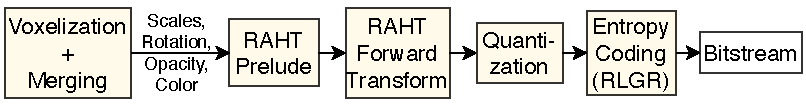
\includegraphics[width=\columnwidth]{figures/raht_pipeline.pdf}
%%     \caption{RAHT coding pipeline.\eduardo{This figure should have the KLT.}}
%%   \label{fig:raht-pipeline}
%% \end{figure}
%% %
%% Because weights are accumulated whenever two coefficients (in sibling pairs) merge, the low-frequency coefficient ends with the largest weight, while high-frequency coefficients produced early have smaller weights.
%% %
%% These weights depend only on the octree structure (not on the attribute values), and thus provide a natural frequency ordering for the coefficients.
%% %
%% Last step is sorting the RAHT coefficients by decreasing weight before quantization and entropy coding; full pipeline in~\cref{fig:raht-pipeline}.
%% %
%% \eduardo{this is not what we do, the ordering is different, I think you explained it earlier in the paper.}

%% \parab{RAHT prelude.}
%% %
%% A naive RAHT implementation would explicitly traverse the octree and discover sibling pairs at each transform step \cite{de2016compression,gpcc}.
%% %
%% This is inefficient since it requires sequential tree traversal.
%% \eduardo{I think this is also inefficient because you do this for ever attribute.  Prelude allows you to figure out all these indices only once, and then you reuse them to apply the RAHT to all attributes. }
%% %
%% Instead, the implementation from~\cite{raht} computes a \emph{prelude} step before running the RAHT transform. 
%% %
%% This finds the indices to per-layer pairs from the morton-ordered voxels.
%% %
%% Concretely, given a voxelized 3D space with morton codes for each voxel, the prelude computes, for each layer $\ell \in \{1,\dots,3J\}$ (3 denotes the number of axes):
%% %
%% (i) an index list $I_\ell$ indicating the active coefficients at that layer,
%% %
%% (ii) a weight list $W_\ell$ for those active coefficients, and
%% %
%% (iii) a flag list $F_\ell$ indicating which active coefficients are left siblings (\ie should be paired with the next coefficient).
%% %
%% Once the prelude $(I_\ell,W_\ell,F_\ell)$ is available, the forward RAHT is just a sequence of independent $2\times2$ matrix-vector products applied to the sibling pairs at each level.

%% \parab{RAHT algorithms.}
%% Before we describe the parallelization, we first explain the RAHT prelude and transform at a high level. The explicit algorithms are presented here~\cref{algo:raht-prelude,algo:raht-forward}.

%% RAHT operates on pairs of sibling voxels, more precisely on the sibling coefficients.
%% %
%% Therefore, at each transform step, RAHT must know which coefficients should be paired and what weights they carry.
%% %
%% A naive implementation would traverse the octree and discover siblings on the fly, but this is sequential and pointer-heavy.
%% %
%% Instead, the RAHT prelude converts the Morton codes for the voxels as indices to the octree.
%% %
%% To recall, the bits of the Morton code for a octree node indicate the path from the root to that node, and also two nodes are siblings if their prefixes match up to a certain bit, given by level $\ell$.
%% %
%% At each step $\ell$, where $1 \le \ell \le 3J$ (3 is due to 3-axes), RAHT prelude computes three lists:
%% %
%% (a) a list of currently active coefficient indices ($I_\ell$),
%% %
%% (b) a boolean indicator that marks which active coefficients are left siblings ($F_\ell$), and
%% %
%% (c) an integer weight per active coefficient ($W_\ell$) that tracks how many leaf voxels are represented by that coefficient.
%% %
%% Intuitively, $I_\ell$ says which coefficients exist at this step, $F_\ell$ says which adjacent coefficients should be paired, and $W_\ell$ provides the pair weights used in Eq.~\ref{eq:raht-butterfly}.
%% %
%% The prelude (Alg.~\ref{algo:raht-prelude}) essentially computes these by scanning adjacent Morton codes: if two adjacent Morton codes share the same prefix at the current step, the earlier one is flagged as a left sibling, and the later one becomes its right sibling; right siblings are then removed to form the next active list.

%% The forward RAHT is a sequence of independent $2\times2$ weighted orthonormal transforms (weights obtained from the prelude) applied to sibling pairs at each step (Alg.~\ref{algo:raht-forward}).
%% %
%% For each left sibling in $F_\ell$, RAHT identifies if its sibling pair exists in the next active coefficient in $I_\ell$, and applies the weighted transform in Eq.~\ref{eq:raht-butterfly} across all attribute dimensions.
%% %
%% This produces one coefficient that is propagated upward (low-frequency) and one coefficient that is kept (high-frequency).
%% %
%% Inverse RAHT transform runs the same steps in reverse order and applies the inverse of Eq.~\ref{eq:raht-butterfly} (the transpose of the forward matrix), reconstructing the attributes.

%% \parab{Why RAHT needs to be parallelized.}
%% A \gs frame has many attribute dimensions: opacity is a scalar, rotation has 4 quaternions, scale has 3 axes, and color has 48 SH coefficients (up to degree 3).
%% %
%% This means that RAHT needs to be applied to each attribute dimension.
%% \eduardo{below I think you should mention across which dimensions you want/can exploit parallelization in raht and prelude, and then say the challenges and how you solve it. I think the parallelizable directions are 1) acrsoss attributes, 2) within each octree level. Across octree levels is sequential, and that introduces the difficulty you describe in more detail below.}
%% \parab{How \gsnfs parallelizes the prelude.}
%% The prelude’s main challenges are (a) sparsity causing irregular sibling structure and (b) the active list shrinking unpredictably across steps.
%% %
%% \gsnfs addresses both with similar \emph{level-synchronous} template for octree parallelization~\cref{sec:octree-encode-gpu}. 
%% %
%% We describe this below:

%% \begin{itemize}
%% \item \textbf{Per-step kernel over a flat list (addresses sparsity).}
%% %
%% At each step $\ell$, \gsnfs maintains the current active list $I_\ell$ as a flat GPU tensor of indices.
%% %
%% We launch one GPU thread per element of $I_\ell$ to compute $W_\ell$ and $F_\ell$.
%% %
%% Each thread compares the Morton code of its current element with the next element (adjacent in Morton order) under the step-specific mask and decides whether they form a sibling pair.
%% %
%% Use of Morton codesdoes not require any octree traversal or pointer chasing for sibling discovery, even though occupancy is sparse.

%% \item \textbf{GPU compaction to form the next list (addresses dynamic list sizes).}
%% After $F_\ell$ is computed, the next active list $I_{\ell+1}$ is obtained by removing right siblings.
%% %
%% \gsnfs implements this efficiently using boolean shift and masked select of tensors which are available in PyTorch (Alg.~\ref{algo:raht-prelude-gpu}).
%% %
%% Note that sometimes we use PyTorch primitives and sometimes we write custom CUDA kernels; the choice is based on efficiency and ease of implementation.
%% %
%% This matches the level-synchronous template: compute on per-element, then compact the list and relaunch.
%% \end{itemize}

%% \parab{How \gsnfs parallelizes the RAHT forward/inverse transform.}
%% At each step $\ell$ going from $1$ to $3J-1$ (bottom up), RAHT must gather the two coefficient rows of each sibling pair, apply a $2\times2$ transform across all attribute dimension, and write results back in-place; steps are sequential, but work \emph{within} a step is parallel.
%% %
%% \gsnfs again follows the level-synchronous template.
%% %
%% At step $\ell$, we launch a GPU kernel with one thread per entry in the active list $I_\ell$.
%% %
%% Only threads whose flag $F_\ell$ is valid execute the $2\times2$ transform; each such thread reads indices of a sibling pair (current and next element in $I_\ell$), looks up their weights in $W_\ell$, computes the two scalar mixing coefficients, and then applies Eq.~\ref{eq:raht-butterfly} to all attribute dimensions.

%% Inverse RAHT uses the same schedule $(I_\ell,F_\ell,W_\ell)$ and the same per-step parallel kernel structure.
%% %
%% The only differences are (i) the order of steps (top-down, i.e., reverse $\ell$) and (ii) using the inverse $2\times2$ transform.
%% %
%% Therefore, the inverse inherits the same parallelization benefits and does not introduce additional structural complexity.

%% \end{comment}
